%%%%%%%%%%%%%%%%%%%%%%%%%%%%%%%%%%%%%%%%%%%%%%%%%%%%%%%%%%%%%%%%%%%
%                                                                 %
%  GEANT manual in LaTeX form                                     %
%                                                                 %
%  Version 1.00                                                   %
%  Last Mod.  8 June 1993 1300   MG                               %
%                                                                 %
%%%%%%%%%%%%%%%%%%%%%%%%%%%%%%%%%%%%%%%%%%%%%%%%%%%%%%%%%%%%%%%%%%%
\Origin{R.Brun}     
\Submitted{01.06.83}   \Revised{26.10.93}
\Version{Geant 3.16}\Routid{BASE200}
\Makehead{Steering routines for event processing}
\Shubr{GRUN}{}
Main routine to control a run of events. The following flow chart is only 
valid for the {\it batch} execution mode. For interactive applications, 
see section {\tt XINT}. A schematic description of the routine is shown 
in fig.~\ref{fg:base200-1}.
 
\begin{figure}[hbt]
      \centering
      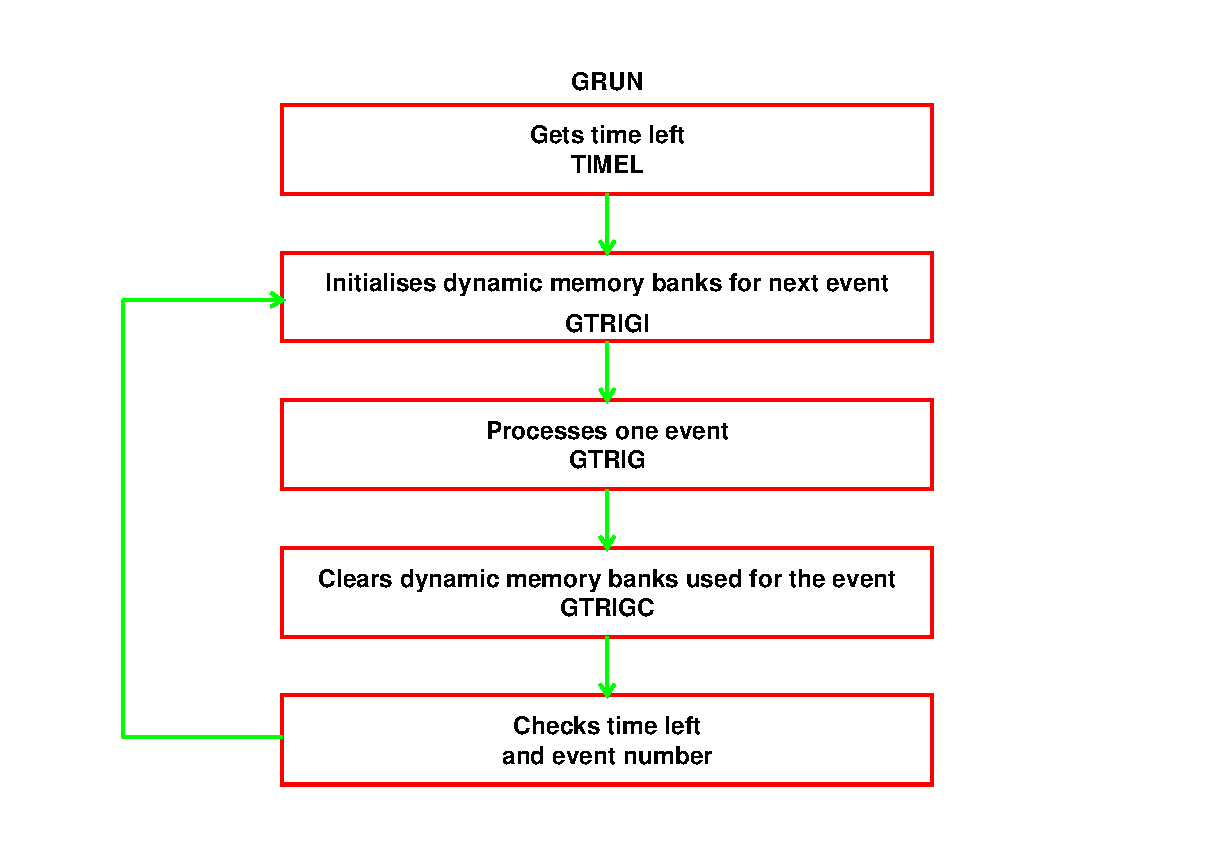
\epsfig{file=eps/base200-1.eps,width=16cm}
      \caption{Flow of the {\tt GRUN} routine.}
      \label{fg:base200-1}
\end{figure}

\Shubr{GTRIGI}{}
Initialisation routine for event processing:
\begin{itemize}
\item resets to 0 the flag {\tt IEOTRI} in \FCind{/GCFLAG/} and the counters
{\tt NTRACK} and {\tt NVERTX} in \FCind{/GCNUM/};
\item sets the debug flag
{\tt IDEBUG} in \FCind{/GCFLAG/}
to the value required for the current event;
\item creates a default header bank
{\tt JHEAD} for current event {\tt [BASE299]};
\item prints the sequence number, the event number and the random number
generator seeds,
under control of the flag {\tt ITEST} (data record {\tt DEBU}).
\end{itemize}
 
\Shubr{GTRIG}{}
 
Steering routine to process one event (trigger).
A schematic description of the routine is shown 
in fig.~\ref{fg:base200-2}.
 
\begin{figure}[hbt]
      \centering
      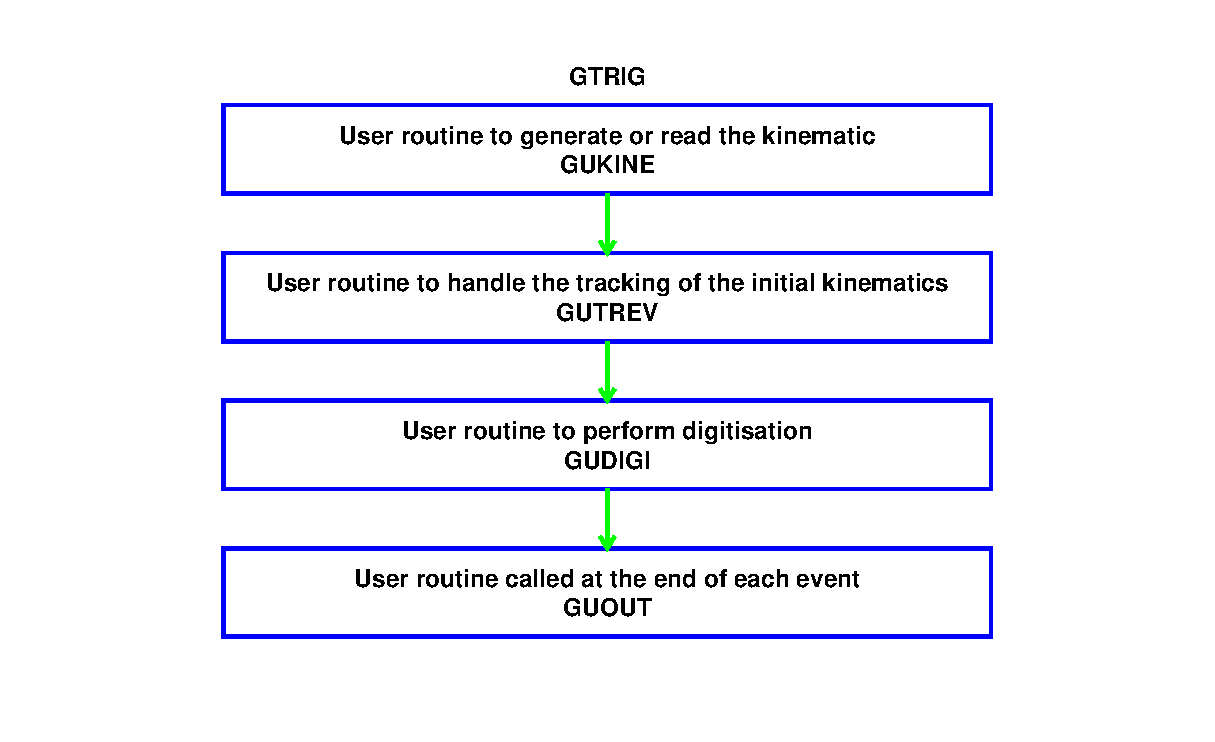
\epsfig{file=eps/base200-2.eps,width=16cm}
      \caption{Flow of the {\tt GRUN} routine.}
      \label{fg:base200-2}
\end{figure}

Default routines provided by {\tt GEANT} are dummy.

\Shubr{GTRIGC}{}
The event division {\tt IXDIV} is cleared. The space
used by the current event may be used by the next one.
 
